%
% This is the LaTeX template file for lecture notes for EE 382C/EE 361C.
%
% To familiarize yourself with this template, the body contains
% some examples of its use.  Look them over.  Then you can
% run LaTeX on this file.  After you have LaTeXed this file then
% you can look over the result either by printing it out with
% dvips or using xdvi.
%
% This template is based on the template for Prof. Sinclair's CS 270.

\documentclass[twoside]{article}
\usepackage{graphics}
\usepackage{graphicx}
\usepackage{algorithm}
\usepackage{mathtools}
\usepackage{mathptmx}
\usepackage{algpseudocode}
\setlength{\oddsidemargin}{0.25 in}
\setlength{\evensidemargin}{-0.25 in}
\setlength{\topmargin}{-0.6 in}
\setlength{\textwidth}{6.5 in}
\setlength{\textheight}{8.5 in}
\setlength{\headsep}{0.75 in}
\setlength{\parindent}{0 in}
\setlength{\parskip}{0.1 in}

%
% The following commands set up the lecnum (lecture number)
% counter and make various numbering schemes work relative
% to the lecture number.
%
\newcounter{lecnum}
\renewcommand{\thepage}{\thelecnum-\arabic{page}}
\renewcommand{\thesection}{\thelecnum.\arabic{section}}
\renewcommand{\theequation}{\thelecnum.\arabic{equation}}
\renewcommand{\thefigure}{\thelecnum.\arabic{figure}}
\renewcommand{\thetable}{\thelecnum.\arabic{table}}

%
% The following macro is used to generate the header.
%
\newcommand{\lecture}[4]{
   \pagestyle{myheadings}
   \thispagestyle{plain}
   \newpage
   \setcounter{lecnum}{#1}
   \setcounter{page}{1}
   \noindent
   \begin{center}
   \framebox{
      \vbox{\vspace{2mm}
    \hbox to 6.28in { {\bf EE 382C/361C: Multicore Computing
                        \hfill Fall 2016} }
       \vspace{4mm}
       \hbox to 6.28in { {\Large \hfill Lecture #1: #2  \hfill} }
       \vspace{2mm}
       \hbox to 6.28in { {\it Lecturer: #3 \hfill Scribe: #4} }
      \vspace{2mm}}
   }
   \end{center}
   \markboth{Lecture #1: #2}{Lecture #1: #2}
   %{\bf Disclaimer}: {\it These notes have not been subjected to the
   %usual scrutiny reserved for formal publications.  They may be distributed
   %outside this class only with the permission of the Instructor.}
   \vspace*{4mm}
}

%
% Convention for citations is authors' initials followed by the year.
% For example, to cite a paper by Leighton and Maggs you would type
% \cite{LM89}, and to cite a paper by Strassen you would type \cite{S69}.
% (To avoid bibliography problems, for now we redefine the \cite command.)
% Also commands that create a suitable format for the reference list.
\renewcommand{\cite}[1]{[#1]}
\def\beginrefs{\begin{list}%
        {[\arabic{equation}]}{\usecounter{equation}
         \setlength{\leftmargin}{2.0truecm}\setlength{\labelsep}{0.4truecm}%
         \setlength{\labelwidth}{1.6truecm}}}
\def\endrefs{\end{list}}
\def\bibentry#1{\item[\hbox{[#1]}]}

%Use this command for a figure; it puts a figure in wherever you want it.
%usage: \fig{NUMBER}{SPACE-IN-INCHES}{CAPTION}
\newcommand{\fig}[3]{
			\vspace{#2}
			\begin{center}
			Figure \thelecnum.#1:~#3
			\end{center}
	}
% Use these for theorems, lemmas, proofs, etc.
\newtheorem{theorem}{Theorem}[lecnum]
\newtheorem{lemma}[theorem]{Lemma}
\newtheorem{proposition}[theorem]{Proposition}
\newtheorem{claim}[theorem]{Claim}
\newtheorem{corollary}[theorem]{Corollary}
\newtheorem{definition}[theorem]{Definition}
\newenvironment{proof}{{\bf Proof:}}{\hfill\rule{2mm}{2mm}}

% **** IF YOU WANT TO DEFINE ADDITIONAL MACROS FOR YOURSELF, PUT THEM HERE:

\usepackage{hyperref}
\hypersetup{
    colorlinks=true,
    linkcolor=blue,
    filecolor=magenta,      
    urlcolor=cyan,
}
 
\urlstyle{same}

\begin{document}
%FILL IN THE RIGHT INFO.
%\lecture{**LECTURE-NUMBER**}{**DATE**}{**LECTURER**}{**SCRIBE**}
\lecture{15}{October 18}{Vijay Garg}{Avin Tung}
%\footnotetext{These notes are partially based on those of Nigel Mansell.}

% **** YOUR NOTES GO HERE:

% Some general latex examples and examples making use of the
% macros follow.  
%**** IN GENERAL, BE BRIEF. LONG SCRIBE NOTES, NO MATTER HOW WELL WRITTEN,
%**** ARE NEVER READ BY ANYBODY.
\section{Introduction}
%Students in EE 382C are required to scribe lecture notes for one lecture.
%These lecture notes will be done using the document processing system called Latex.
%We have posted the file {\em scribe.tex} on the Canvas system. You can run {\tt pdflatex}
%on that file to generate {\em scribe.pdf}. The remaining document shows usage of
%some of the commands in Latex.
\indent This lecture will complete the Cuda examples and begin covering algorithms for parallel programming using GPU: 
\begin{enumerate}
	\item reduce.cu 
	\item Parallelism Vocabulary 
	\item Blelloch Scan 
	\item Brick Sort
\end{enumerate}


\section{reduce.cu}
Check out the Cuda code for \href{https://github.com/vijaygarg1/UT-Garg-EE382C-EE361C-Multicore/blob/master/cuda/reduce.cu}{reduce.cu} [1].

It uses multiple blocks, each with multiple threads, of the GPU to compute the sum of the array by reduction. It splits the array into multiple section for each block to sum using its multiple threads. When each block is complete with its portion, a single block will sum the final sums and return. 

Each block runs the following code. The code splits the array in half, then uses n/2 threads to sum entries n+i and n+i+(n/2) for i= 0 to n/2 into a new array of size n/2. Before the next iteration, \emph{syncthreads} function is called to make sure all adds are done before moving on. This is repeated until there is only one entry left which is the sum of the total array. The new value is then written back to global with a single thread. 

The key things to note is the program runs a global memory kernel in data and a shared memory kernel in sdata. This example is to show the difference in time between threads running using global memory and threads running on their own shared memory. 


\section{Parallelism Vocabulary}
There are specific terms that are often used when talking about writing programs for GPUs.
\\
\\
\\
\subsection{Map}
Map maps every entry to another entry, one to one, and returns it. So for every i, we return it's corresponding f(i). In terms of parallelism, it can be done in O(1) time depending on the complexity of the mapping function.  

\begin{figure}[ht]
  \centering
  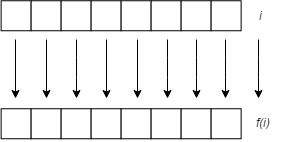
\includegraphics[width=0.50\textwidth]{./Mapping.png} 
  \caption{Mapping}
  \label{fig:map}
\end{figure}

\subsection{Reduce}
Reduce is taking an associative operator applied to multiple entries and reducing it to one- many to one. The important thing to note is to understand the identity of the operation. For example, the values for sum should be initialized to 0, the values for max should be initialized to -\infinity, the values for min should be initialized to \infinity, and so on. 

\begin{figure}[ht]
  \centering
  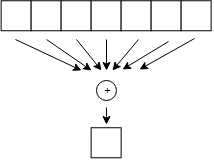
\includegraphics[width=0.50\textwidth]{./Reduce.png} 
  \caption{Reduce with Add Operation}
  \label{fig:reduce}
\end{figure}
\\
\\
\\
\\
\\
\\
\subsection{Scan}
Scan takes an array and creates a new array such that the new array's element j is the sum of all the elements before j and including/excluding j. If we include j, it is classified as an inclusive scan, and if j is excluded, then it is an exclusive scan. This is also known as the prefix sum.

\begin{figure}[ht]
  \centering
  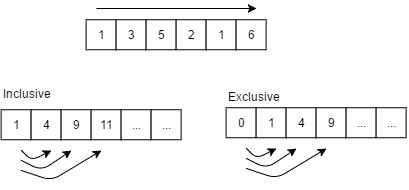
\includegraphics[width=0.50\textwidth]{./Scanning.png} 
  \caption{Scan}
  \label{fig:scan}
\end{figure}

\subsection{Scatter}
Scatter takes an array scatters the entries into a new array. An example of scatter can be merging two sorted arrays into one sorted array using binary search to calculate the new address into the new array. 

\begin{figure}[ht]
  \centering
  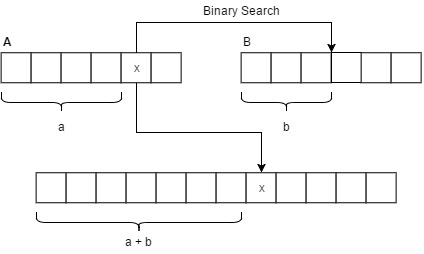
\includegraphics[width=0.50\textwidth]{./Scatter.png} 
  \caption{Scatter Example: Merging Two Sorted Arrays}
  \label{fig:scatter}
\end{figure}

\subsection{Gather}
Gather takes multiple entries and does a sequence of operations to them to reduce it to one entry- many to one. The key thing about gather is that some synchronization and atomicity may be used depending on the sequence of operations. For example, we can take 3 entries, and average them into one entry in a new array. This requires an atomic add for each of the 3 entries as well as a barrier before dividing it by 3.   

\begin{figure}[ht]
  \centering
  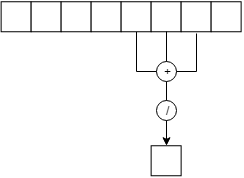
\includegraphics[width=0.50\textwidth]{./GatherAverage.png} 
  \caption{Gather Example: Average Example}
  \label{fig:gather}
\end{figure}

\subsection{Transpose}
Transpose is moving memory from one piece position in memory to another, or liken to transposing a matrix. This is useful in parallel programming since it moving entries into memory that is faster to access and operate on, such as into local cache, can significantly improve the performance time.

\subsection{Stencil}
Stencil is like the 3D version of gather. If on a matrix of entries, stencil can take multiple entries surrounding the desired entry, operate on them, and store the value into a new grid of entries. 

\begin{figure}[ht]
  \centering
  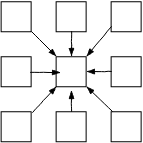
\includegraphics[width=0.25\textwidth]{./Stencil.png} 
  \caption{Stencil}
  \label{fig:stencil}
\end{figure}

\subsection{Compact}
Compact is looking at an array, operate on it, and return a compact version of the original array. For example, an array can have multiple threads reading each entry and test whether it is prime, and return only the prime values into a new, smaller array. 

\begin{figure}[ht]
  \centering
  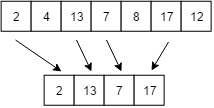
\includegraphics[width=0.25\textwidth]{./Compact.png} 
  \caption{Compact Example: Prime}
  \label{fig:compact}
\end{figure}

\section{Blelloch Scan}
Blelloc Scan is used to find the total sum of all entries while being both work optimal as well as time efficient. The speed and work is summarized and compared to other total scan sum algorithms we have discussed previously. 

\begin{centering}
\begin{tabular}{ |p{8cm}||p{3cm}|p{3cm}|p{3cm}|  }
 \hline
 \multicolumn{3}{|c|}{Scan Algorithm Complexities} \\
 \hline
Scan Algorithm & Time Complexity & Work Complexity\\
 \hline
 Sequential Scan & O(n) & O(n)\\
 Parallel Prefix Scan (Hillis-Steele) & O(logn)& O(nlogn)\\
 Blelloch Scan & O(logn) & O(n) \\
 \hline
\end{tabular}
\end{centering}


For Blelloch Scan, there are two phases to compute the exclusive scan- an upsweep and a downsweep. In the upsweep phase, we do a sum operation on each neighboring pair, keeping track of each of the summed intermediate entries for reference for the downsweep phase. Once the upsweep phase is complete, we set the last node we touch to 0. We then follow it with the downsweep phase, such that at each level we take the previous left entry and add it to the current entry and set that to its new right entry, and carry the current entry to the new left entry.  

Upsweep can be computed as:
\begin{equation}sum[v] = sum[L[v]] + sum[R[v]]
\end{equation}
Downsweep can be computed as:
\begin{equation}
\begin{split}
scan[L[v]] = scan[v] \\
scan[R[v]] = sum[L[v]] + scan[v]
\end{split}
\end{equation}

Where \emph{sum[L[v]]} is the most recent, nearest, unused summed left value during the upsweep phase.


The parallelism exist since each pair addition is done by an independent thread. 

See bottom of document for Blelloch Scan Example 

\begin{figure}[!h]
  \centering
  \framebox{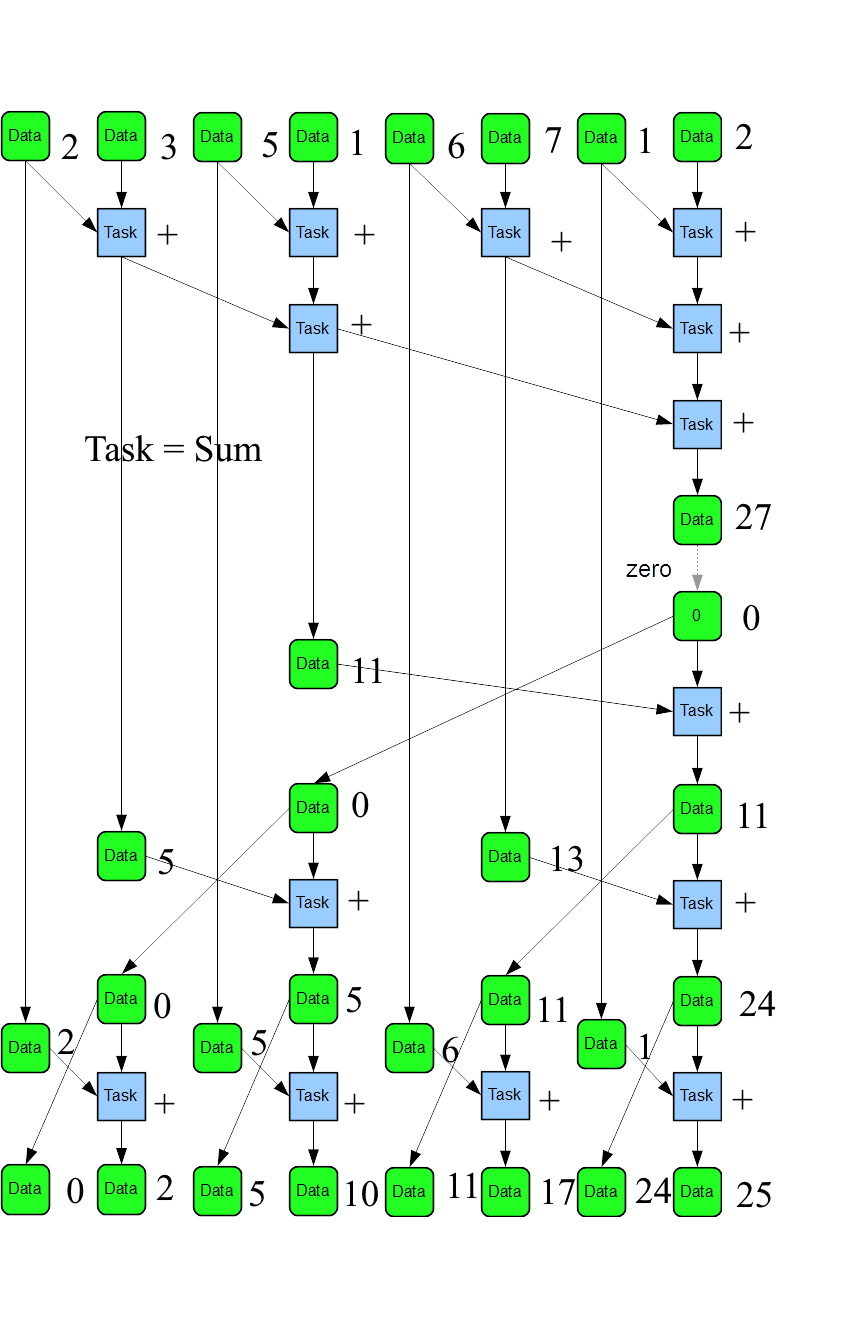
\includegraphics[width=0.75\textwidth]{./prefix-scan-balanced.png}}
  \caption{Blelloch Scan [4]}
  \label{fig:Bleloch}
\end{figure}

\section{Brick Sort (Odd-Even Sort)}
Brick sort sorts an array of entries like bubble sort with parallelism. It breaks the array into pairs, then compares (and swaps) all pairs into order. Then, on the new array, the entries pair off with the neighbor it did not previously pair with, and repeat. Each pair comparison is handled by an independent thread. This process will take n pairings to complete, therefore O(n).

\begin{figure}[h]
  \centering
  \framebox{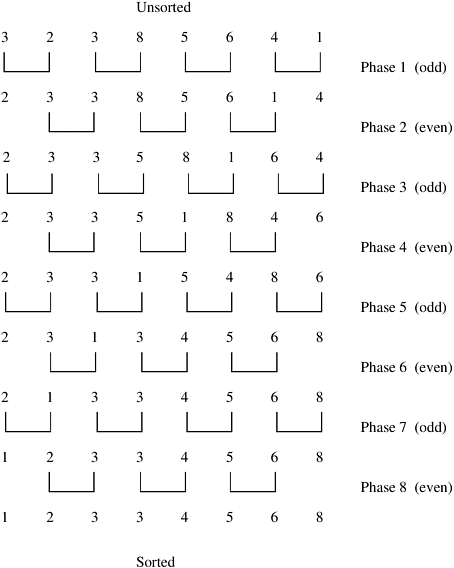
\includegraphics[width=0.50\textwidth]{./Even-Odd-Sort.jpg}}
  \caption{Brick Sort [2]}
  \label{fig:Even-Odd-Sort}
\end{figure}


\begin{figure}[!h]
  \centering
  \framebox{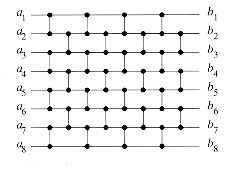
\includegraphics[width=0.50\textwidth]{./Network.jpg}}
  \caption{Brick Sort Network View [3]}
  \label{fig:Network}
\end{figure}

Brick sort is easy to implement, but is an oblivious sorting algorithm. This means it does not take the values into account and will always take the same amount of time based on the number of entries in the array. Furthermore, brick sort can be viewed as a sorting network, where the entries are the input to the network, and the output will be the sorted entries. In the following figure, the vertical lines are comparators and the horizontal lines are the wire the entries can travel across. The a's are the initial entries and the b's are the sorted entries.\newpage\newpage\newpage\clearpage
\section*{References}
\beginrefs
\bibentry{1} https://github.com/vijaygarg1/UT-Garg-EE382C-EE361C-Multicore/blob/master/chapter3-
\\synchronization\_primitives/BoundedBufferMonitor.java
\endrefs
\beginrefs
\bibentry{2} http://d1gjlxt8vb0knt.cloudfront.net//wp-content/uploads/Even-Odd-Sort.gif
\endrefs
\beginrefs
\bibentry{3} http://staff.ustc.edu.cn/~csli/graduate/algorithms/book6/651\_a.gif
\endrefs
\beginrefs
\bibentry{4} https://scs.senecac.on.ca/~gpu621/pages/images/prefix-scan-balanced.png
\endrefs


\end{document}




